% --- Program Section ---

\newprogram{Program 1}{Implement search(nums: List[int], target: int) -> int and myPow(x: float, n: int) ->
float functions taking an integer array/target and base/exponent pairs, returning index and computed
value respectively.}

\subsection*{Code}


\begin{lstlisting}[language=python]
from typing import List

# 1. Search in Rotated Sorted Array
def search(nums: List[int], target: int) -> int:
    left, right = 0, len(nums) - 1

    while left <= right:
        mid = (left + right) // 2

        if nums[mid] == target:
            return mid

        # Left half is sorted
        if nums[left] <= nums[mid]:
            if nums[left] <= target < nums[mid]:
                right = mid - 1
            else:
                left = mid + 1

        # Right half is sorted
        else:
            if nums[mid] < target <= nums[right]:
                left = mid + 1
            else:
                right = mid - 1

    return -1


# 2. Power Function - x^n
def myPow(x: float, n: int) -> float:
    if n == 0:
        return 1.0

    # Handle negative exponent
    if n < 0:
        x = 1 / x
        n = -n

    result = 1.0

    # Binary exponentiation
    while n > 0:
        if n % 2 == 1:
            result *= x

        x *= x
        n //= 2

    return result

if __name__ == "__main__":
    nums = [-1, 0, 3, 5, 9, 10]
    target = 5
    print("Index:", search(nums, target))
    print("Power:", myPow(2.0, 9))
    print("Power:", myPow(4.0, -2))

\end{lstlisting}

\subsection*{Output}
\begin{center}
    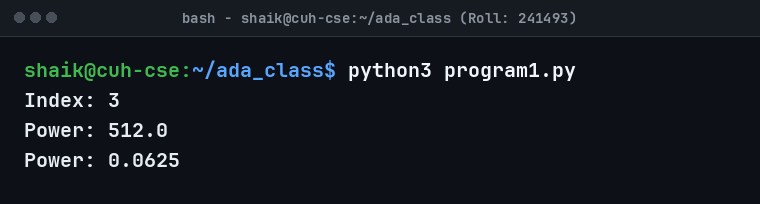
\includegraphics[width=0.88\textwidth]{Images/output_screenshot1.png}
\end{center}

\subsection*{GitHub Scan Code}
\begin{center}
    \begin{minipage}{0.3\textwidth}
        \centering
        % Generates a 2.5cm high QR code directly linking to the code file
        \qrcode[height=3.5cm]{https://github.com/gytdrop/ada_class/blob/main/program1.py} \\[0.2cm]
        \scriptsize\ttfamily Scan to view source code 
    \end{minipage}
\end{center}


% Add a horizontal line that indicates the END of the program.
\vspace{1cm}
\begin{center}
    \rule{1\textwidth}{1pt} % Clean, centered 1pt thick horizontal line
\end{center}